\chapter{Representation Configuration} \label{chapter:Representation Configuration}
\section{Introduction}
Programming languages are textual, and so require a keyboard In order to edit programs. Standard on-screen keyboards are inconvenient for texting, let alone for programming. In addition, they take almost one third of the screen which makes the small screen even smaller. In order to avoid using the inconvenient on-screen keyboard or an external device, we suggest to program by voice. Voice dictation is based on a common set of templates; these templates are individually customizable so that each developer can use the idioms that are most convenient for him or her.

We describe the idea of programming in natural language by writing requirements in order to bridge the gap between the code that the programmer wants to write and a code that is written on the screen. We claim that natural language can serve as the main tool for programming. We do not claim that it is the only tool, the programmer may use other gestures such as touch, on-screen keyboard, or external devices when he needs them.

\section{Configuration}
We suggest that every programmer will dictate his program the way is more convenient to him or her. Every one of us has a different way of describing the things that s/he want to say. Same with code dictation.

For example take the Java loop in \autoref{fig17}. We would dictate it character by character: "for, open parenthesis, int, space etc.". This is inconvenient and cumbersome. Instead, we would like to forget about the syntax and just describe what you want. One way to say it is: "for i from zero to n". But other programmer may prefer to say "repeat n times" to describe the same loop.

We don't just dictate code from top to bottom; we also need to edit existing code and navigate to specific places in the code. Navigation depends on the context of what is shown on the screen, and on the surrounding code. For example, if the screen contains only one loop, I can say "Go to the loop". Or I could say "Rename the index of the first loop to j" to navigate to the first loop on the screen and change its index variable. This demonstrates that templates used for dictation has named parts, and I can refer to these parts when I issue editing or navigation commands.
\begin{figure}[H]
\begin{lstlisting}
for(int i = 0; i < n; i++)
\end{lstlisting}
\caption{A simple for loop}
\label{fig17}
\end{figure}
\section{Natural Language Processing}
In-order to process dictation we suggest two phase process: converting speech to text, and understanding the context of the text. We use speech to text engine for the speech conversion and context free grammar to understand the  context.
\subsection{Speech To Text Engines}
We found several speech to text engines that we can use for our solution: Nuance Dragon \cite{Nuance14} is a software developer kit (SDK) is used by developers and integrators to add speech recognition capabilities into in-house and commercial applications or workflow applications. This toolkit, which enables everything from free-text dictation to command and control functionality, can be deployed as part of a server- or client-based solution; Kaldi \cite{Povey_ASRU2011} is a toolkit for speech recognition written in C++ and licensed under the Apache License v2.0. Kaldi is intended for use by speech recognition researchers. Google Speech Server V2 \cite{google15} is a an online free speech to text engine which runs on a server. Mostly used by researchers. We decided to use Google Speech Server V2 because it is free and easy to use. There are much more speech to text engines but we decided to concentrate on the most known and the one that we choose to use.
\subsection{Context Free Grammar}
A context-free grammar (CFG) is a tuple $ G=(T,N,S,R) $, where $ T $ is the finite set of  terminals of the language, $ N $ is the set of non-terminals that represent phrases in a sentence, $ S \in N $ is the start variable used to represent a full sentence in the language. $ R $ is the set of production rules of the form $ N \rightarrow (N \bigcup T)* $.
\subsubsection{Extended Backus Naur Form}
Extended Backus Naur Form is a notation for formally describing syntax how to write entities in language. The metalanguage is based on a suggestion by Niklaus Wirth (Wirth, 1977) that is based on Backus-Naur Form and that contains the most common extensions, i.e:
\begin{itemize}
	\item Terminal symbols of the language are quoted so that any character,
	including one used in Extended BNF, can be defined as a terminal symbol of
	the language being defined.
	\item $ [ $ and $ ] $ indicate optional symbols.
	\item $ \{ $ and $ \} $ indicate repetition.
	\item Each rule has an explicit final character so that there is never any
	ambiguity about where a rule ends.
	\item Brackets group items together. It is an obvious convenience to use ( and ) in their ordinary mathematical sense.
\end{itemize}
\subsection{Dictation Parser}
We use EBNF to create a set of rules that will validate commands that the programmer dictates. This set of rules can be extended easily by every user that understand EBNF. We use IEEE\\IEC EBNF \cite{IEEEBNF1996} as our main reference to learn how to use EBNF. In \cite[pages 51-86]{Michal2009} Michal Gordon and David Harel claim that formal structured natural language requirements can serve as the mean and the end to programming the behavior of reactive system using fully executable languages such as live sequence charts (LSC). We adopt this approach and use it to create a set of rules to process user dictation.

\subsubsection{Grammar Construction}
We now show how our grammar translates controlled natural language. Since we allow a CFG we can increment the grammar with additional rules that allow various ways of generating similar constructs. We can thus increase the set of accepted specifications by augmenting the grammar. However, ambiguity may grow as the grammar grows which would require the user to explicitly disambiguate his intentions in too many cases for the process to be friendly. We shall describe how basic commands such as: creation, navigation, and modification are parsed. The \textit{Dictation Parser} tries to build a parse tree for every dictation that it receives. A valid dictation is a one that the \textit{Diction Parser} succeeded to create a parse tree for. A number of advanced ideas are not yet supported in the current implementation. Nevertheless, the current grammar allows implementing fully executable systems, and has been tested, among other examples, on the \textit{LinkList} Example, and on the \textit{Command Pattern} Example, see \ref{subsection: Grammar Testing}.

The set of rules is divided into three main layers: \textit{Top}, \textit{Categories}, and \textit{Common}. The \textit{Top} layer contains rules that have access to all categories. The Categories layer contains sub sections that divided to different categories. For example, the \textit{Creation} sub section contains all rules that deal with creation. The \textit{Common} layer knows nothing about any category, it contains all the necessary information for all actions. The \textit{Top} layer and the \textit{Categories} layer have access to the \textit{Common} layer. \autoref{fig19} shows how rules divided into layers and sub categories. Note that this division has no effect on the action of rules. It is only to understand the set of rules better.

We now shall explain every sub category inside the \textit{Categories} layer. \textit{Creation} contains all rules that parse any creation dictation. For example, "Create a new class". \textit{Navigation} contains all rules that parse any navigation dictation. For example, "Go to class person". \textit{Modification} contains all rules that parse any modification dictation.

We now discuss two dictations that have the same meaning but expressed differently. It is important to Deverywhere to allow programmers dictate code in their preferred way. Lets assume that the programmer created a class \textit{Car} and now he wants to create an inner class \textit{Wheel}. One way to say it is \textit{"create a static public class named wheel inside class car"}. \autoref{fig21} presents the parse tree that is generated for this dictation. This dictation will lead to creating a new  static class called \textit{Wheel} inside a class that is called \textit{Car}.

\begin{figure}[H]
\centering
\includegraphics[scale=0.4]{"./fig/Parse Tree create a static public class named wheel inside class car"}
\caption{The parse tree for the sentence "create a static public class named wheel inside class car".}
\label{fig21}
\end{figure}

Another way to say it is \textit{"create an inner class wheel"}. In this case the class that will be create won't be static and the cursor of the IDE shall be placed inside class \textit{Car}, otherwise the class \textit{Wheel} won't be created inside class \textit{Car}. \autoref{fig22} presents the parse tree that is generated for this dictation. This dictation will lead to creating a new class called \textit{Wheel} inside a class that is called \textit{Car}.

\begin{figure}[H]
\centering
\includegraphics[scale=0.4]{"./fig/Parse Tree create an inner class wheel"}
\caption{The parse tree for the sentence "create an inner class wheel".}
\label{fig22}
\end{figure}

\begin{figure}[H]
\centering
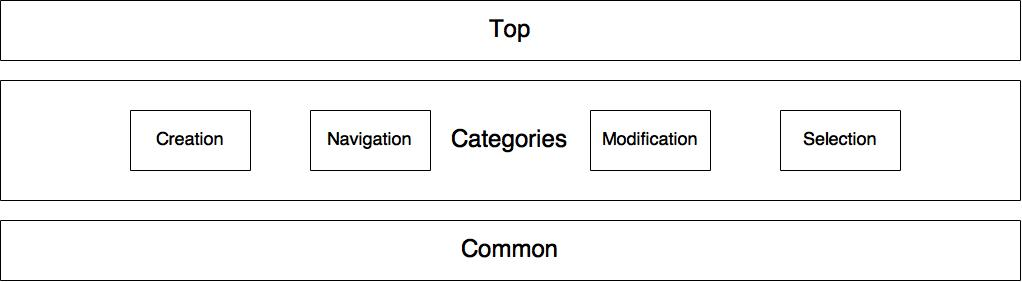
\includegraphics[scale=0.4]{./fig/BNFDiagram}
\caption{This is the architecture of the Dictation Parser rules}
\label{fig19}
\end{figure}
\autoref{tab11}
\begin{table}[H]
	\centering
	\label{my-label}
	\begin{tabular}{|p{10cm}|p{6cm}|}
		\hline
		\rowcolor[HTML]{9B9B9B} 
		{\color[HTML]{000000} Rule} & {\color[HTML]{000000} Description} \\ \hline
		<Command> ::= <Creation-Command> | <Navigation-Command> | <Modification-Command> | <Selection-Command>& bla \\ \hline
		<Creation-Command> ::= <Creation-Verb> [(an | a)] (<Create-Statement> | <Create-Data-Type> | <Create-Field> | <Create-Method> | <Create-Block>) [<Element-Location>]&     \\ \hline
		&     \\ \hline
		&     \\ \hline
	\end{tabular}
	\caption{}
	\label{tab11}
\end{table}

\begin{figure}[H]
	\begin{lstlisting}
	for(int i = 0; i < n; i++)
	\end{lstlisting}
	\caption{A simple for loop}
	\label{fig20}
\end{figure}

\subsection{Grammar Testing} \label{subsection: Grammar Testing}
To test the grammar we provide two programs and their transcripts. The first example is an implementation of a linked list and the second is an example of the Command design pattern. 
\subsubsection{LinkedList Example}
This is an implementation of the data structure linked list. \autoref{fig23}-\autoref{fig29} presents the program that implements Linked List. \autoref{itemize:LinkedList Dictation} lists the dictations that generates this program.
\begin{figure}[H]
	\begin{lstlisting}
	public class LinkedList implements Iterable {
	    private Node head;
	    private Node tail;
	    private int size;
	    
	    public Iterator iterator(){
	        return new LLIterator();
	    }
	    
		private class Node{
			public Object data;
			public Object next;
			
			public Node(Object data, Object next){
				this.next = next;
				this.data = data;
			}
			
			public Object getNext(){
				return next;
			}
			
			public Object getData(){
				return data;
			}
			
			public void setNext(Object next){
				this.next = next;
			}
		}
	\end{lstlisting}
	\caption{Implementation of Linked List in Java part 1}
	\label{fig23}
\end{figure}
\begin{figure}[H]
	\begin{lstlisting}
	    private class LLIterator implements Iterator{
	        private Node nextNode;
	        private boolean removeOK;
	        private int posToRemove;
	        
	        private LLIterator(){
	            nextNode = head;
	            removeOK = false;
	            posToRemove = -1;
	        }
	        
	        public boolean hasNext(){
	            return nextNode != null;
	        }
	        
	        public Object next(){
	            assert hasNext();
	            
	            Object result = nextNode.getData();
	            nextNode = nextNode.getNext();
	            
	            removeOK = true;
	            posToRemove++;
	            
	            return result;
	        }
	\end{lstlisting}
	\caption{Implementation of Linked List in Java part 2}
	\label{fig24}
\end{figure}
\begin{figure}[H]
	\begin{lstlisting}
	        public void remove(){
	            assert removeOK;
	            removeOK = false;
	            LinkedList.this.remove(posToRemove);
	            posToRemove--;
	        }
	    }
	    
	    public void makeEmpty(){
	        head = tail = null;
	        size = 0;
	    }
	    
	    public Object remove(int pos){
	        assert pos >= 0 && pos < size;
	        Object result;
	        if( pos == 0 ){
	            result = head.getData();
	            head = head.getNext();
	            if( size == 1 )
	                tail = null;
	        }
	        else{    
	            Node temp = head;
	            for(int i = 1; i < pos; i++)
	                temp = temp.getNext();
	            result = temp.getNext().getData();
	            temp.setNext( temp.getNext().getNext() );
	            if( pos == size - 1)
	                tail = temp;
	        }
	        size--;
	        return result;
	    }
	    
	    public Object get(int pos){
	        assert pos >= 0 && pos < size;
	        Object result;
	        if( pos == size - 1 )
	            result = tail.getData();
	        else{
	            Node temp = head;
	            for(int i = 0; i < pos; i++)
	                temp = temp.getNext();
	            result = temp.getData();
	        }
	        return result;
	    }
	    
	    public void insert(int pos, Object obj){
	        assert pos >= 0 && pos <= size;
	        if(pos == 0)
	            addFirst(obj);
	
	        else if( pos == size )
	            add(obj);
	        else{
	            Node temp = head;
	            for(int i = 1; i < pos; i++)
	                temp = temp.getNext();
	
	            Node newNode = new Node(obj, temp.getNext());
	            temp.setNext( newNode );
	            size++;
	        }
	    }
	    
	    public void add(Object obj){
	        Node newNode = new Node(obj, null);
	        if( size == 0 )
	            head = newNode;
	        else
	            tail.setNext(newNode);
	        tail = newNode;
	        size++;
	    }
	    
	    public void addFirst(Object obj){
	        if(size == 0)
	            add(obj);
	        else{
	            Node newNode = new Node(obj, head);
	            head = newNode;
	            size++;
	        }
	    }
	    
	    public String toString(){
	        String result = "";
	        Node temp = head;
	        for(int i = 0; i < size; i++){
	            result += temp.getData() + " ";
	            temp = temp.getNext();
	        }
	        return result;
	    }
	}
	\end{lstlisting}
	\caption{Implementation of Linked List in Java part 3}
	\label{fig25}
\end{figure}
\begin{figure}[H]
	\begin{lstlisting}
	        public void remove(){
	            assert removeOK;
	            removeOK = false;
	            LinkedList.this.remove(posToRemove);
	            posToRemove--;
	        }
	    }
	    
	    public void makeEmpty(){
	        head = tail = null;
	        size = 0;
	    }
	\end{lstlisting}
	\caption{Implementation of Linked List in Java part 4}
	\label{fig26}
\end{figure}
\begin{figure}[H]
	\begin{lstlisting}
	    public Object remove(int pos){
	        assert pos >= 0 && pos < size;
	        Object result;
	        if( pos == 0 ){
	            result = head.getData();
	            head = head.getNext();
	            if( size == 1 )
	                tail = null;
	        }
	        else{    
	            Node temp = head;
	            for(int i = 1; i < pos; i++)
	                temp = temp.getNext();
	            result = temp.getNext().getData();
	            temp.setNext( temp.getNext().getNext() );
	            if( pos == size - 1)
	                tail = temp;
	        }
	        size--;
	        return result;
	    }
	\end{lstlisting}
	\caption{Implementation of Linked List in Java part 5}
	\label{fig27}
\end{figure}
\begin{figure}[H]
	\begin{lstlisting}
	    public Object get(int pos){
	        assert pos >= 0 && pos < size;
	        Object result;
	        if( pos == size - 1 )
	            result = tail.getData();
	        else{
	            Node temp = head;
	            for(int i = 0; i < pos; i++)
	                temp = temp.getNext();
	            result = temp.getData();
	        }
	        return result;
	    }
	    
	    public void insert(int pos, Object obj){
	        assert pos >= 0 && pos <= size;
	        if(pos == 0)
	            addFirst(obj);
	
	        else if( pos == size )
	            add(obj);
	        else{
	            Node temp = head;
	            for(int i = 1; i < pos; i++)
	                temp = temp.getNext();
	
	            Node newNode = new Node(obj, temp.getNext());
	            temp.setNext( newNode );
	            size++;
	        }
	    }
	\end{lstlisting}
	\caption{Implementation of Linked List in Java part 6}
	\label{fig28}
\end{figure}
\begin{figure}[H]
	\begin{lstlisting}
	    public void add(Object obj){
	        Node newNode = new Node(obj, null);
	        if( size == 0 )
	            head = newNode;
	        else
	            tail.setNext(newNode);
	        tail = newNode;
	        size++;
	    }
	    
	    public void addFirst(Object obj){
	        if(size == 0)
	            add(obj);
	        else{
	            Node newNode = new Node(obj, head);
	            head = newNode;
	            size++;
	        }
	    }
	    
	    public String toString(){
	        String result = "";
	        Node temp = head;
	        for(int i = 0; i < size; i++){
	            result += temp.getData() + " ";
	            temp = temp.getNext();
	        }
	        return result;
	    }
	}
	\end{lstlisting}
	\caption{Implementation of Linked List in Java part 7}
	\label{fig29}
\end{figure}
This is the list of the dictations that generates the program.
\begin{itemize} \label{itemize:LinkedList Dictation}
	\item Create class LinkedList that implements Iterable
	\item Create private field head of type Node
	\item Create private field tail of type Node
	\item Create private field size of type int
	\item Create method iterator that returns Iterator
	\item Return new LLIterator
	\item Exit method iterator
	\item Create inner class Node
	\item Create field data of type Object
	\item Make it public
	\item Create public field next of type Object
	\item Create constructor that accepts data of type Object and next of type Node
	\item Assign next to this.next
	\item Assign data to this.data
	\item Create method getNext that returns Object
	\item Return next
	\item Create method getData that returns Object
	\item Return data
	\item Create method setNext that accepts next of type object
	\item Assign next to this.next
	\item Exit class Node
	\item Create inner class LLIterator that implement Iterator
	\item Create a constructor
	\item Assign head to field nextNode	
	\item Assign false to field removeOK
	\item Assign -1 to field posToRemove
	\item Ceate method hasNext that returns boolean
	\item Return is nextNode different from null
	\item Ceate method next that return Object
	\item Assert hasNext
	\item Create result of type object and assign nextNode.getData to it
	\item Call nextNode.getNext and assign it to nextNode
	\item Assign true to removeOK
	\item Increase posToRemove
	\item Return result
	\item Create method remove
	\item Assert removeOK
	\item Assign false to removeOK
	\item Call LinkedList.this.remove that accepts posToRemove
	\item Decrease posToRemove
	\item Exit LLIterator
	\item Crete method makeEmpty
	\item Assign null to tail and head
	\item Assign zero to size
	\item Create method remove that accept pos of type int and returns Object
	\item Assert is pos more than 0 and pos less than size
	\item Create result of type Object
	\item If pos equal to 0 then
	\item Call head.getData and assign it to result
	\item Call head.getNext and assign it to head
	\item If size equal 1 then
	\item Assign null to tail
	\item Exit the if
	\item Else
	\item Create temp of type Node and assign head to it
	\item For i from 1 to pos
	\item Call temp.getNext and assign it to temp
	\item Exit the loop
	\item Call temp.getNext.getData and assign it to result
	\item Call temp.setNext that accepts temp.getNext.getNext
	\item If pos equal size minus 1 then
	\item Assign temp to tail
	\item Exit else
	\item Decrease size
	\item return result
	\item Create method get that accepts pos of type int and returns Object
	\item Assert is pos more or equal to 0 and less than size
	\item Create result of type Object
	\item If pos equal size minus 1 then
	\item Call tail.getData and assign it to result
	\item Else
	\item Create temp of type Node and assign head to it
	\item For i from 0 to pos
	\item Call temp.getNext and assign it to temp
	\item Exit for
	\item Call temp.getData and assign it to result
	\item Exit else
	\item Return result
	\item Create method insert that accepts pos of type int and obj of type Object
	\item Assert is pos more or equal to 0 and less than size
	\item If pos equal to 0 then
	\item Call addFirst that accepts obj
	\item Else if pos equal size then
	\item Call add that accepts obj
	\item Else
	\item Assign head to temp of type Node
	\item For i from 1 to pos
	\item Call temp.getNext and assign it to temp
	\item Exit the for loop
	\item Create new Node that accepts obj and temp.getNext and assign it to newNode of type Node
	\item Call temp.setNext that accept newNode
	\item Increase size
	\item Exit method insert
	\item Create method add that accepts obj of type Object
	\item Create new Node that accepts obj and null and assign it to newNode of type Node
	\item If size equal 0 then
	\item Assign newNode to head
	\item Else
	\item Call tail.setNext that accepts newNode
	\item Exit
	\item Assign newNode to tail
	\item Increase size
	\item Create method addFirst that accepts obj of type Object
	\item If size equal 0 then
	\item Call add that accepts obj
	\item Else
	\item Create new Node that accepts obj and head and assign it to newNode of type Node
	\item Assign newNode to head
	\item Increase size
	\item Create method toString that returns String
	\item Create result of type String and initialize it with an empty string
	\item Assign head to temp of type Node
	\item For i from 0 to size
	\item Result plus equal temp.getData plus space
	\item Call temp.getNext and assign it to temp
	\item Exit the loop
	\item Return result
\end{itemize}
\subsubsection{Car Builder Example}
This is an implementation of the Builder design pattern. We created a class of type Car that have properties and contains an inner class of type CarBuilder that has the functionallity to create an instance of Car. In-addition it has main. \autoref{fig30}-\autoref{fig31} presents the program that implements Linked List. \autoref{itemize:Car Builder Dictation} lists the dictations that generates this program.
\begin{figure}[H]
	\begin{lstlisting}
	public class Car
	{
		private String _wheels;
		private String _engine;
		private String _body;
	
		private Car(String wheels, String engine, String body)
		{
			if(body == null || engine == null || wheels == null)return;
	
			_wheels = wheels;
			_engine = engine;
			_body = body;
		}
	
		public static class CarBuilder
		{
			String Body;
			String Wheels;
			String Engine;
			public Car BuildCar()
			{
				if(Body != null && Wheels != null && Engine != null)
				{
					return new Car(Wheels, Engine, Body);
				}
				return null;
			}
		}
	\end{lstlisting}
	\caption{Implementation of the design pattern Builder that creates a class of type Car part 1}
	\label{fig30}
\end{figure}
\begin{figure}[H]
	\begin{lstlisting}
		public static void main(String[] args)
		{
			Car.CarBuilder carBuilder = new CarBuilder();
			carBuilder.Engine = "honda";
			carBuilder.Wheels = "4";
			carBuilder.Body = "private";
			Car car;
			car = carBuilder.BuildCar();
		}
	}
	\end{lstlisting}
	\caption{Implementation of the design pattern Builder that creates a class of type Car part 2}
	\label{fig31}
\end{figure}
This is the list of the dictations that generates the program.
\begin{itemize} \label{itemize:Car Builder Dictation}
	\item Create class car
	\item Create field wheel of type string
	\item Create field engine of type string
	\item Create field body of type string
	\item Create private constructor that accept wheels of type string engine of type string and body of type string
	\item If body equals null or engine equals null or wheels equals null then return	
	\item Assign wheels to field wheels
	\item Assign engine to field engine
	\item Assign body to field body
	\item Create inner class CarBuilder
	\item Create public field body of type string
	\item Create public field wheels of type string
	\item Create public field engine of type string
	\item Create method buildCar that returns Car
	\item If body different from null or wheels different from null or engine different from null then return new car that accepts wheels engine and body
	\item Return null
	\item Create main inside car
	\item Create new CarBuilder and assign it to carBuilder of type carBuilder
	\item Assign honda as string to carBuilder.engine
	\item Assign 4 as string to carBuilder.engine
	\item Assign private as string to carBuilder.engine
	\item Create car of type car
	\item Call carBuilder.BuildCar and assign it to car
\end{itemize}
\section{Implementation}
To implement the \textit{Dictation Parser} we reviewed different applications such as: BNFC, BNF Parser Generator, BNF for Java, Antlr 4. We decided to use Antlr 4 because it is can be integrated well in our solution, popular and well-known tool and it is well known to other members of the team. The implementation of the \textit{Dictation Parser} is explained in details in \ref{section:BNF Parser}.